%!TEX root = cscw2019-comic.tex
\section{Discussion}
\label{sec:Discussion}
Here we first summarize our findings from the study studies. Then we will propose a framework for algorithmically synthesizing persuasive messages into the abstract comic form, the limitation of the study, and the future research directions. 

%need to update this part after the revision of RQ in the introduction
%Our experiment answers RQ-1 affirmatively in that comics are more persuasive than text, with a moderate effect of 0.33. Our answer to RQ-2 is that while the effect of no element is significant, shading and gesture show strong influence, but surprisingly inter-character distance is most effective when distance is large. For RQ-3, we show that negative messages are more influential than positive messages. We have developed a prototypical comic generator (answering RQ-4) that can be used in deploying comic messages.

In the collective action dilemma, persuading individuals to cooperate or contribution is crucial. Since the public good is a good that is both non-excludable and non-rivalrous, individuals can benefit from the goods without contribution. The free-ride problem will eventually lead public goods to scarce. So, nudging individuals to vote, volunteer time, give to political or charitable organizations, and donate blood is important. In our study, we looked at a novel form of the persuasive message, abstract comic, and examined its effect in persuading people to make charitable donations. Our results show that study participants prefer persuasive messages in comic form over plain text in collective action decisions with the real cost. When making the charitable donation between $\$0$ to $\$5$, study participants donated $\$ 0.75$ more if they read the persuasive message in an abstract comic form. The results demonstrate the persuasive power of abstract comic in nudging people to engage in pro-social behavioral decisions. Our findings are consistent with prior research on visual stimulus in persuasion and the benefits of comics in communication. One potential explanation is that study participants were more attracted by the comic strip and projected themselves onto the character. When the projection happens, the persuadee may be able to digest the information better which nudged them to donate more to the OAR. However, when comparing between the comic condition and comic+social condition, although study participants who read the comic with 'social proof' donated more, our analysis result did not imply meaningful effect size. Although the use of 'social proof' showed a significant impact on other forms of persuasive messages (e.g. pure textual), in the abstract comic persuasive messages, the effect is not substantial. One of the potential explanation is that the design of our comic strip did not signify the idea of 'social proof' other than in the text bubble. It is worth to explore other comic designs, e.g. adding other donators as comic characters, that can make the 'social proof' more salience. Although in our study, the persuasive goal is contributing to public goods, we believe our finding can be generalized to other persuasive scenarios such as behavioral change.

\subsection{Model Selection}
\label{sub:Model Selection}

As in any task with modeling data, one can reasonably ask about the validity of our choices for the model. For example, how useful was the choice of the Student-t drawing distribution~\Cref{eq:bayesian formulation}, instead of assuming that the outcomes are drawn from a Normal distribution? It is easy to do a Bayesian analysis and we can show that when we use a Normal drawing distribution instead of a Student-t, there is negligible effect on the results, the contrasts and the effect sizes are nearly identical, with marginal effect on the HPD width for the Posterior distributions. This is consistent with the estimate of the degrees of freedom $\nu=53$ (c.f.~\Cref{fig:robustcontrasts}); since $\nu \geq 30$ is the usual criterion for using Normal distributions.

A more interesting case is the use of a bounded distribution like a $Y \sim Beta(\alpha, \beta)$ distribution to represent the charitable donations under the different conditions; This is reasonable, since the charitable donations are bounded by experimental design to lie between \$0.0 and \$5.0. While a $Beta(\alpha, \beta)$ distribution lies between $[0,1]$, we can scale down the contributions to lie in $[0,1]$ to use with the $Beta(\alpha, \beta)$ distribution. But notice from~\Cref{fig:contributions across conditions} that in each experimental condition, there is a central lobe, and heavy tails at each extreme, notably at \$0 and at \$5. While we can use a $Y \sim Beta(\alpha, \beta)$ distribution to model charitable contributions, it is easy to examine the Posterior prediction check (a figure similar to~\Cref{fig:posteriorprediction} for a model with a $Beta(\alpha, \beta)$ distribution) for the case of the $Y \sim Beta(\alpha, \beta)$ distribution to see that the tails of the distributions for each experimental condition are not modeled well. 

% followed Our analysis shows that subjects prefer persuasive messages in comic form over plain text. We found in a persuasive comic, different character's gestures and background shading can influence subjects' perception of the persuasiveness whereas no strong effect was found in inter-character distance. This was consistent with previous research on visual stimulus in persuasion and the benefits of comics in communication.
%
% \subsection{Inter-Character Distance}
% \label{sub:Inter-Character Distance}
% There may be two explanations to the odd result that the farthest distance between the two characters was more influential.
% % However, previous studies on comics composition suggests the inter-character distance can affect reader's perceived relationship between characters and therefore influence their perception of the persuasive comics.
% First, it may be the case that the subjects did not project themselves onto the comic as one of the characters and did not recognize the distance between characters as reflecting closeness of the relationship. For example, a subject may read the comic from a third-person narrative. We looked into some feedbacks from in the pilot study. One participant ($p_1$) mentioned \textit{``I really like the comic I just saw and I feel bad that someone told me ...''} which suggests the subject does think that they are in the comic and having a conversation with someone else. Yet, we don't know if they perceive their relationship with the persuader based on the inter-character distance. A second explanation is that closer inter-character distance causes a cluttered visual composition and thus the subjects perceive these comics as less visually pleasing.

% \subsection{Comics with Color}
% \begin{figure}[t]
%  \centering
%  \begin{tabular}{ccc}
%   \subfloat[Colored Text]{\label{figur:3o}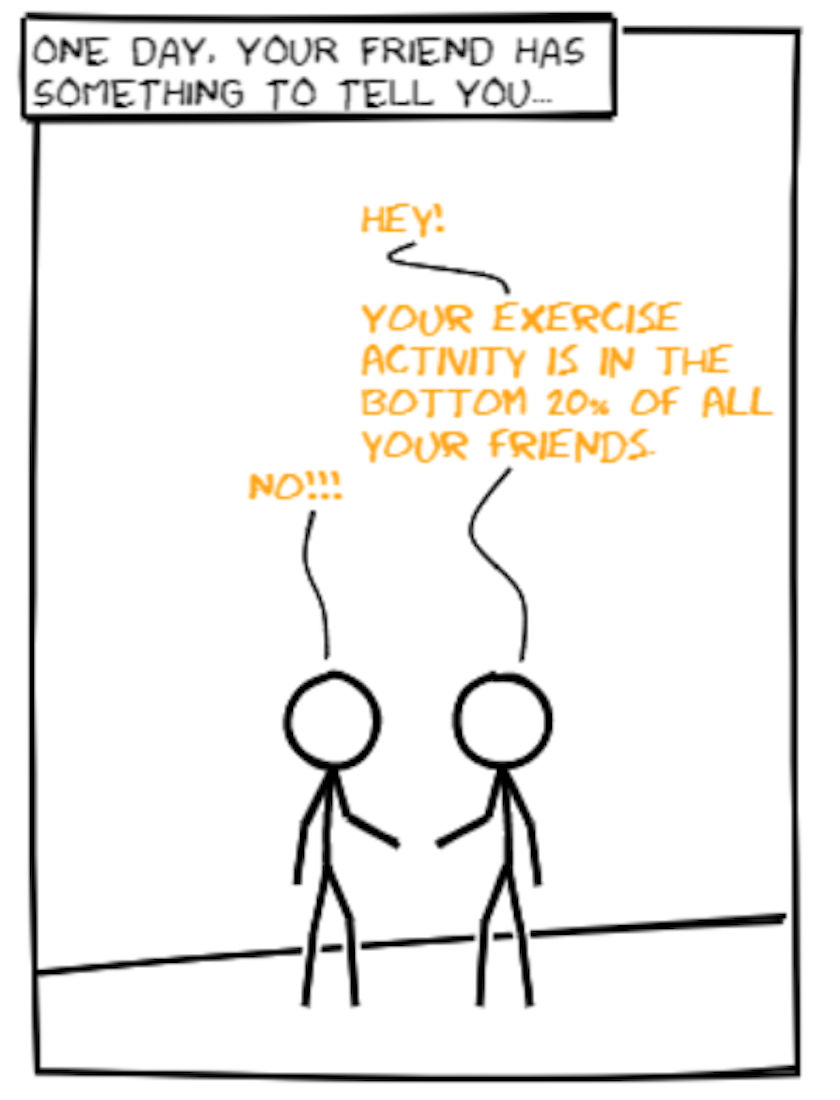
\includegraphics[width = 0.27\columnwidth]{figures/o1}} &
%   \subfloat[Colored Ground Line]{\label{figur:31}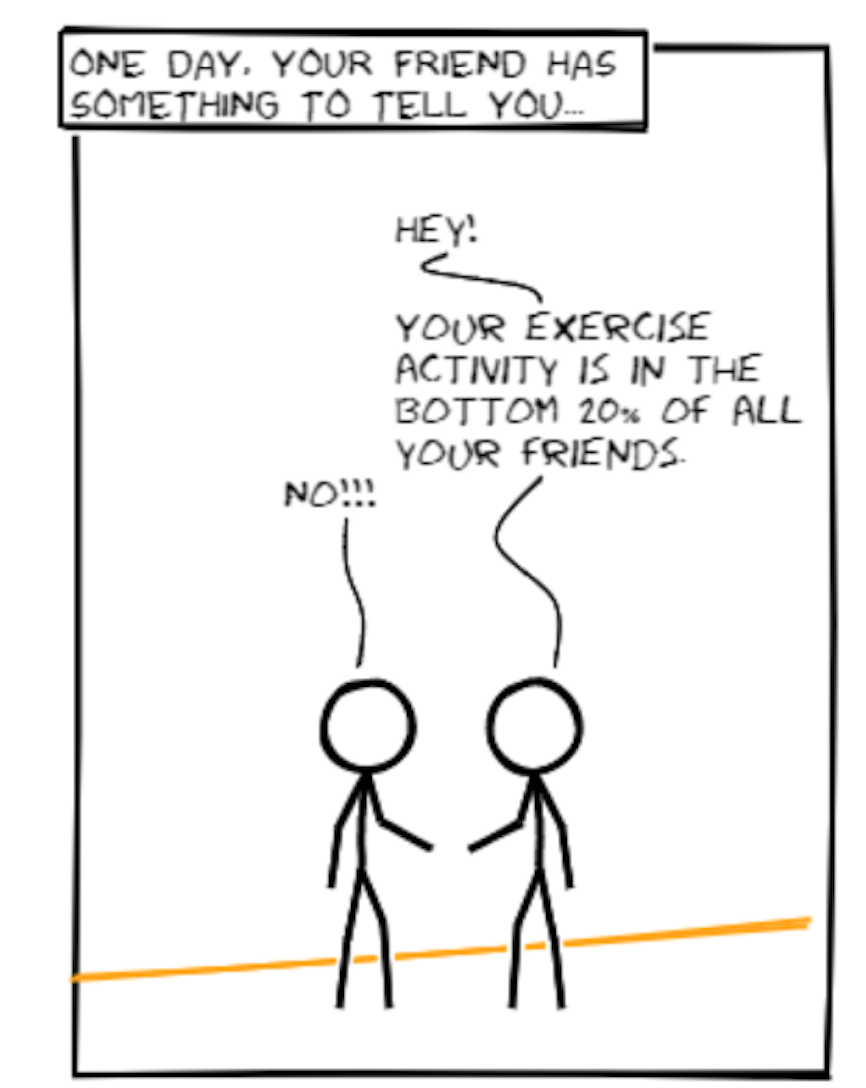
\includegraphics[width = 0.27 \columnwidth]{figures/o2}}      &
%   \subfloat[Colored Figure]{\label{figur:32}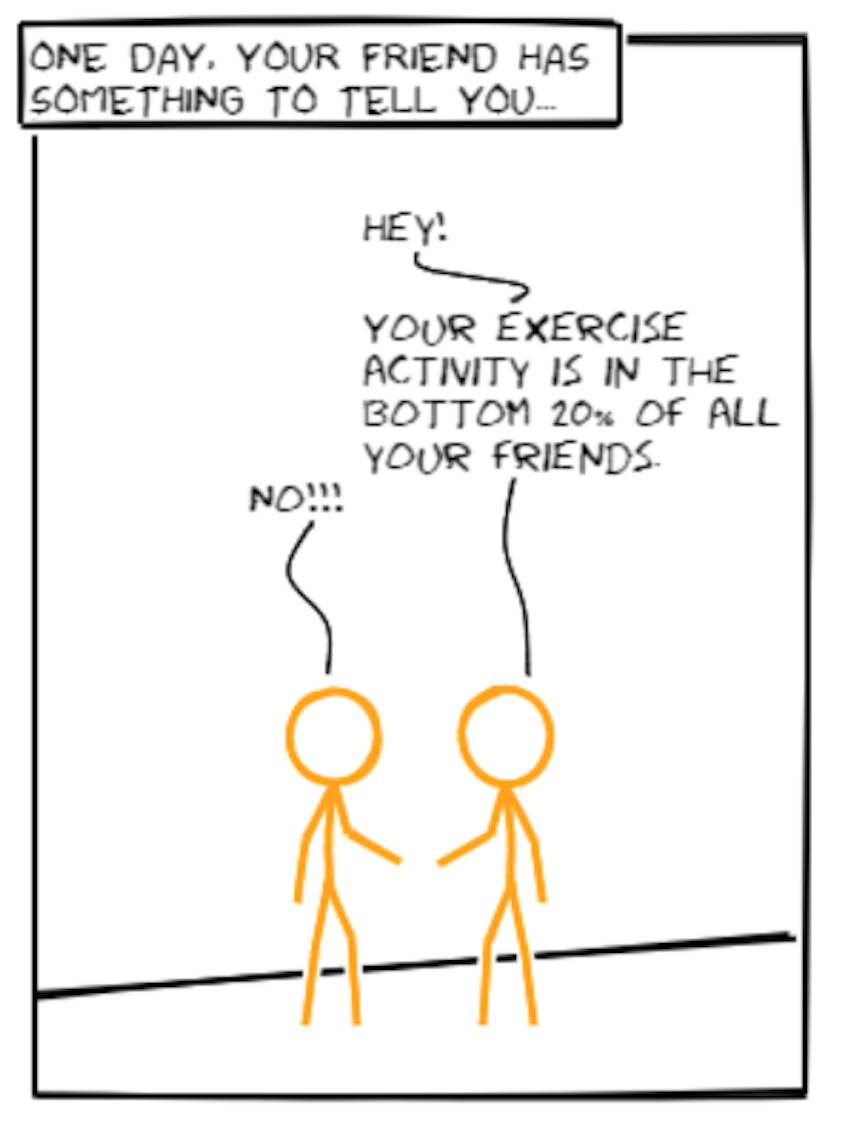
\includegraphics[width = 0.27 \columnwidth]{figures/o3}}\\
%  \end{tabular}
%  \caption{Colored different elements in a comic}
%  \label{figur:color}
% \end{figure}
%
% Our model suggests the background shading in a persuasive comic affects its persuasive power which makes us wonder the role of color as previous studies suggest the usage of color communicates the emotional intensity similar to the background shading. We ran a small scale study comparing the perceived persuasiveness between black-white comics in our study and their corresponding colored version,see figure~\ref{figur:color}. With 60 participants from the Mechanical Turk,  we found using an identical hierarchical Bayesian formulation that our subjects perceive colored version as more persuasive and there is potential interaction effect between negative-positive framing and different colors (see~\Cref{fig:color-experiment-effect}). We plan to run larger experiments that include color and study the interaction with framing and other elements.
%
% \begin{figure}
%  \subfloat[The mean effect and the effect size with color\label{subfig-1:color-mean-effect}]{%
%   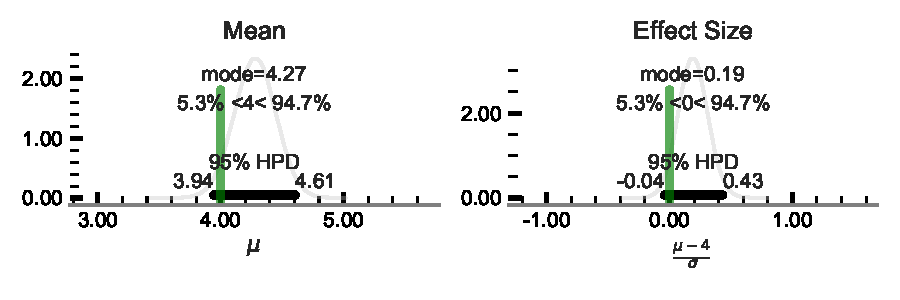
\includegraphics[width=0.6\textwidth]{./hari-code/factors_mean_effect_color-no-interaction.pdf}
%   } \hfill
%  \subfloat[Color contrast\label{subfig-2:color-contrast}]{%
%   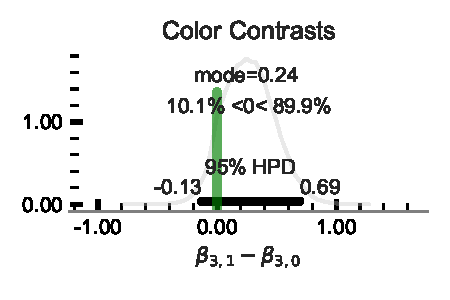
\includegraphics[width=0.33\textwidth]{./hari-code/factors_color_contrasts_color-no-interaction.pdf}
%  }
%  \caption{~\Cref{subfig-1:color-mean-effect} shows the High Posterior Density (HPD) intervals for the mean response $\mu$ and effect sizes $\sigma_y$ in the presence of color. HPD represent the region with 95\% of the density. Notice that the HPD interval for $\mu$ is $[3.94, 4.27]$ and includes a ROPE of $[4\pm 0.1]$ (the interval includes 4, the neutral response value). Thus while there no significant effect, we note that nearly 94\% of the HPD lies to the right of 0. The figure for effect size shows a small effect with mode $0.19$; since the HPD interval $[-0.04, 0.43]$ includes a ROPE of $[0\pm 0.1]$, there is no significant effect.~\Cref{subfig-2:color-contrast} shows the contrasts between the use of the two colors. The modal value is $0.24$, but since the HPD interval $[-0.13, 0.69]$ overlaps with 0, there is no appreciable effect (but notice that 89\% of the density lies in the region greater than 0.)}
%  \label{fig:color-experiment-effect}
% \end{figure}

\subsection{Limitations}
\begin{description}
%  \item[No interaction effects in model]: Our model does not include any interaction effects. This is by design, since in the first study we have 54 experimental conditions making the any analysis interaction effects difficult with our small observational study. The raw data suggests an interaction between shading and gesture, but given our limited dataset, there is little point in modeling this interaction. We plan to study interaction effects in future studies by limiting the number of main predictor conditions.
 \item[Generalizability:]  Although our study asked participants to make decision with cost, the decision domain is limited to only one scenario, charitable giving. We need more studies to evaluate persuasiveness of abstract comics in other domains.

 \item[Ecological Validity:] There is a legitimate question if our experiment on Amazon Mechanical Turk has ecological validity.  In real life, many factors  affect a persons decision, such as where they are and who they are interacting with. Those factors may interact with the abstract comic's persuasiveness. However, these concerns are also present in other standard studies conducted in the more familiar lab experiments. We plan to conduct field studies in real-world contexts (e.g. shopping at a grocery store) to explore this issue.
  
 \item[Comic Construction:] Although the XKCD style is one of the most popular abstract comic styles, there were thousands of ways to create abstract comics. Also, the complexity our comics strip (e.g. number of characters, gestures, and the number of panels) is limited. While simplicity grants us the possibility to automate the generation process, future technology may allow us to generate more complicated persuasive abstract comics. Therefore, it is valuable to understand the persuasiveness of other abstract persuasive comics.
\end{description}
%  Large scale field study is needed to demonstrate how the abstract comic can persuade in the real-life decision making and what will affect its persuasiveness.
 %Since we ask the subjects (who may lack interest in exercise) to evaluate persuasiveness when the topic is on exercise. Notice that our goal is not to persuade experimental subjects to exercise more, but to evaluate if the comic is a more persuasive form of communication of a statistical fact. We should expect---since we don't know if the subjects are interested in exercise---an increase in the variance in the estimates of the parameters (in particular,  $\sigma_y$). Despite this, the analysis shows a significant affirmative result for RQ-1.
%  \item[Appropriate gestures]: The authors determined gestures used by the characters in the experiment through trial and error. It may be useful to examine  theoretical frameworks from dance as well as theater art forms as well as examine work on design of sign languages.
% \end{description}
 % \item[Single Panel]: Our experiment limits our comics to a single panel which hinders one of the most fascinating aspect of comics---storytelling. Comparing to the comic strip, single panel comics find it harder to show the dynamic among characters.

 \subsection{Framework for Algorithmically Synthesized Abstract-Comic Persuasive Messages}
 Our study showed the persuasive power of abstract comics in encouraging people to make pro-social decisions. However, one drawback of using visual stimulus in persuasion is the creation process. Comparing to the pure-textual form, generating abstract comics costs more. In this section, we propose a framework that allows full/semi- automatic generation of abstract persuasive messages. We believe such a tool will lower the barrier for the persuader to take advantage of the abstract comic (as demonstrated in our study) in encouraging individuals to participate in collective actions.

 In our study, we created a comic generator with existing packages such as cmx.io and rough.js to generate the three panel abstract comic strip. With several pre-defined character gestures (see~\Cref{figur:figures}), the generator only requests the text input from the persuader.  

 We believe the generator we built can be further developed as a framework for algorithmic synthesis: the behavioral data informs the text and character gestures. We could derive the statistics for the social norm from behaviors of friends and the data from a person's own activity for information framing, and map the data to the character gesture, thus reinforcing the framing. While both information framing and the use of social proof improve the comic persuasiveness, our studies indicate the comic form is more important. Thus, we expect the comic form to be useful, even if behavioral data or social norms are unavailable.

\begin{figure}[t]
	\centering
	\begin{tabular}{cc}
		\subfloat[Gestures for positive framed messages]{\label{figur:1a}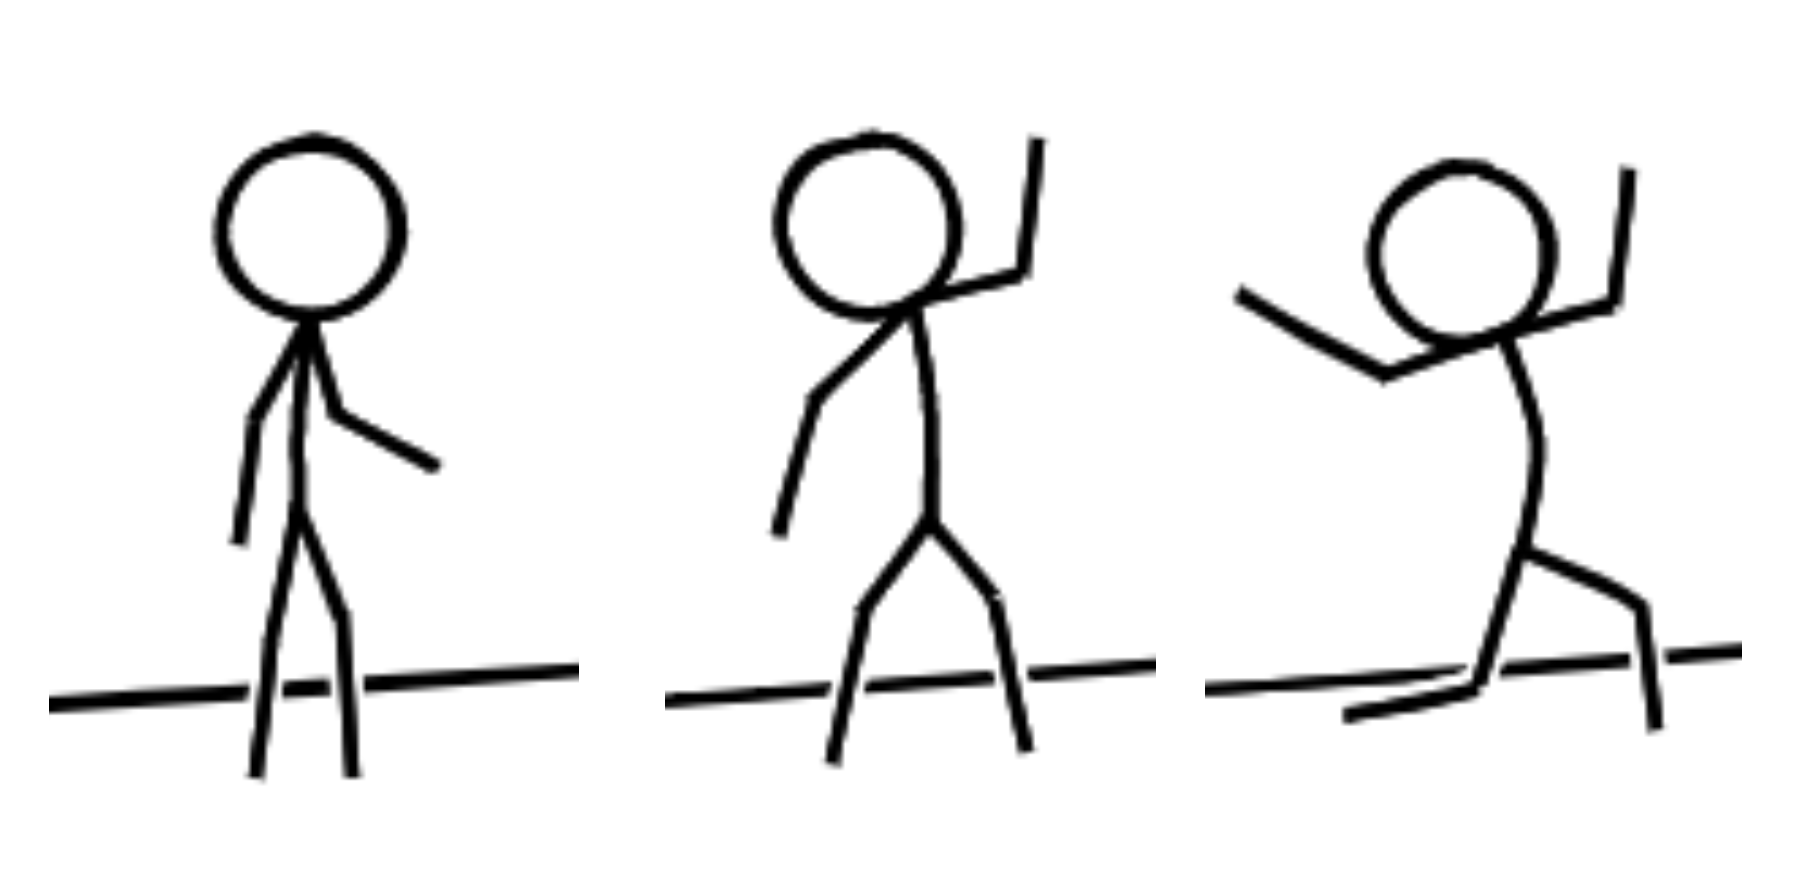
\includegraphics[width = 0.4\columnwidth]{figures/pos_figures}} &
		\subfloat[Gesture for negative framed messages ]{\label{figur:1b}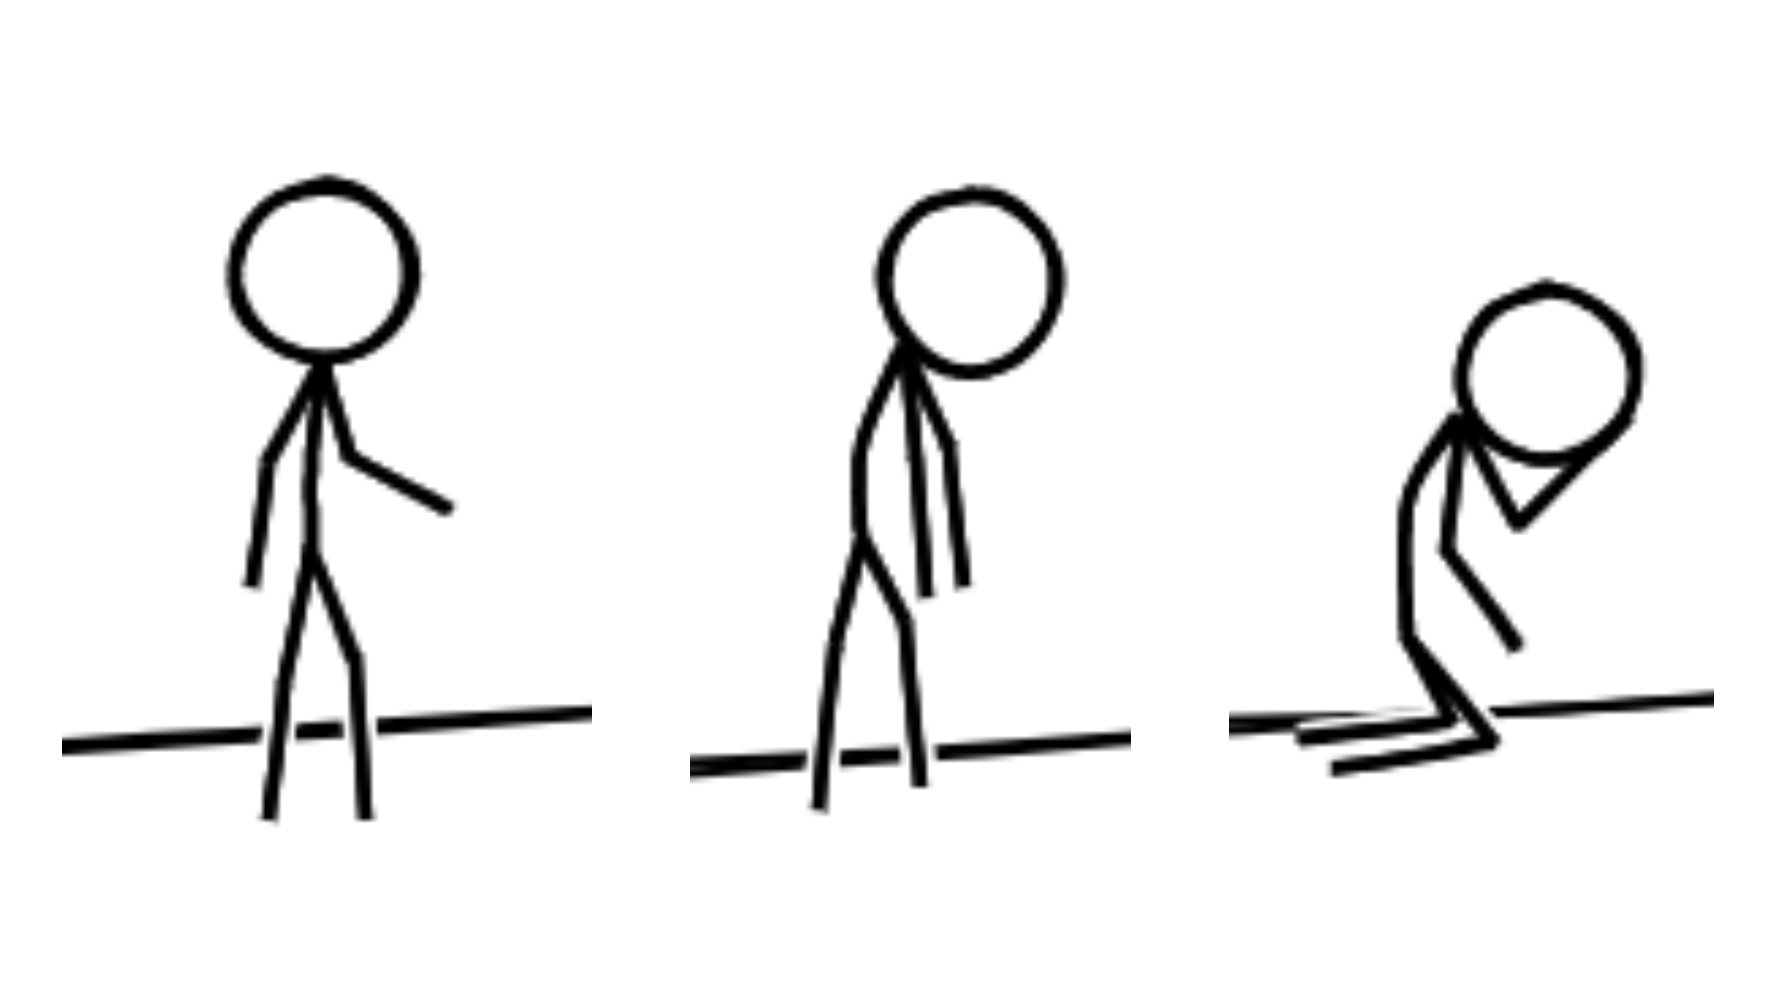
\includegraphics[width = 0.4 \columnwidth]{figures/neg_figures}}\\
	\end{tabular}
	\caption{Different character gestures to communicate various levels of emotional intensity. The left figure shows gestures from neutral to the happiest. The right figure shows gestures from neutral to the most frustrated. }
	\label{figur:figures}
\end{figure}

\subsection{Future Research}
The main implication of our study lies in how to deliver persuasive messages. Given the increasing popularity of wearable devices including smartwatches, one could consider presenting persuasive messages in the form of an abstract comic, where the three-panel comic is shown in sequence, perhaps even in animation. 

Also, ~\textcite{scott1993understanding} identifies several fundamental components that influence reader reaction: character gestures, inter-character distance, and shading intensity. For example, the gesture of a character can help the reader to understand the interaction between characters and the emotion of the character. As a common technique, cartoonists often use the gesture to intensify the feeling that they want to communicate to the reader \cite{scott1993understanding}. Therefore, one of the future direction should be understanding how the different comic components moderate comic persuasiveness. If different comic elements car persuades differently, taking advantage of data-driven methods, the abstract-comic can better persuade. To maximize the persuasive power, future research on computational persuasion should leverage the receiver's personal model to construct the persuasive abstract comics with elements best fit to the persuadee.